\chapter{GUI}
Il passo successivo alla costruzione del sistema intelligente è stato lo sviluppo della GUI da rendere l'utilizzo più facile a utenti non esperti da riga di comando, facilitando quello che è il workflow.\\
L'interfaccia è stata costruita in modo tale da avere un'unica pagina con molteplici tab, posizionate in ordine di utilizzo, per rendere meno dispersivo e più intuitivo possibile il sistema creato. Le sezioni in ordine sono le seguenti:
\begin{itemize}
	\item Home
	\item Classify
	\item Predict
	\item Merge
	\item Settings
\end{itemize}

Come specificato nell'introduzione per questa parte si è utilizzato il linguaggio di programmazione Python con un modulo per la realizzazione della grafica chiamato PyQt. Tale modulo altro non è se non un binding del noto framework cross-platform QT per C++. A differenza del linguaggio appena citato, Python non gode della stessa velocità di esecuzione dal momento che si tratta di un linguaggio interpretato, ma ha come punto di forza la facilità di sviluppo.

\section{Home}
Appena avviato il programma si presenta nel modo seguente fornendo una breve introduzione su che cosa sia il programma in utilizzo e illustrando brevemente le sue modalità di lavoro.
\begin{figure}[h!]
	\begin{center}
		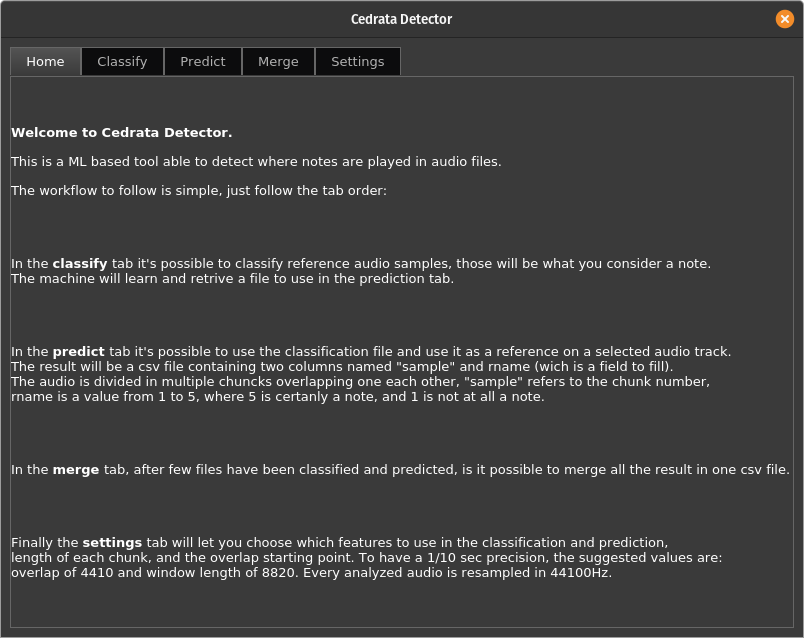
\includegraphics[scale=0.5]{./immagini/gui/home.png}
	\end{center}
	\caption{Schermata di home}\label{fig:gui-home}
\end{figure}

\section{Classify}
Procedendo con quello che l'ordine delle sezioni arriviamo alla prima vera e propria sezione, quella per lo svolgimento della classificazione, dove viene costruito un file ARFF che verrà, nel punto successivo, utilizzato per la costruzione di un classificatore. Sono richiesti in input: una cartella contenente tutti i campioni di note per cui si vorranno estrarre le features, il nome della relazione, in questo caso lo strumento di cui si stanno effettuando le estrazioni, e in fine una cartella di destinazione per salvare il file ARFF creato avente come nome il nome della relazione.
\begin{figure}[h!]
	\begin{center}
		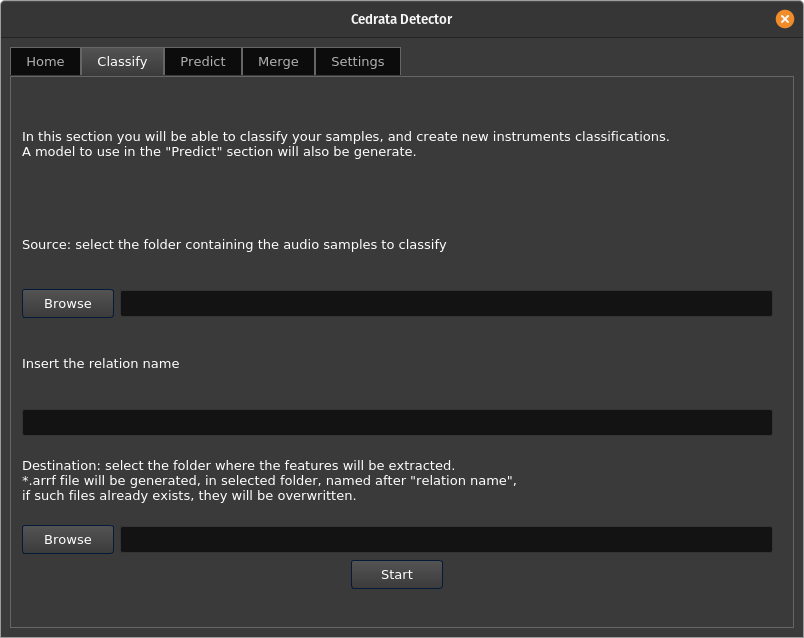
\includegraphics[scale=0.5]{./immagini/gui/classify.png}
	\end{center}
	\caption{Schermata di home}\label{fig:gui-classify}
\end{figure}

\section{Predict}
A questo punto l'utilizzatore avrà ottenuto un file ARFF dalla sezione precedente, tale viene richiesto in input per costruire un classificatore assieme a un file audio nei formati AIFF o WAV. Per terminare sarà necessario indicare la directory dove salvare i risultatati scritti in un file di tipo CSV (Comma-Separated value) il quale presenterà due colonne, sub-sample e note. Le tracce audio verranno infatti trattate allo stesso modo di quelle usate per la classificazione, creando così dei sub-sample, di lunghezza e overlap specificati nelle impostazioni del software, con i rispettivi valori delle features associati. A ogni sub-sample verrà associata una classe di nota, da 1 a 5, e quindi stampata nel file CSV risultante.
\begin{figure}[h!]
	\begin{center}
		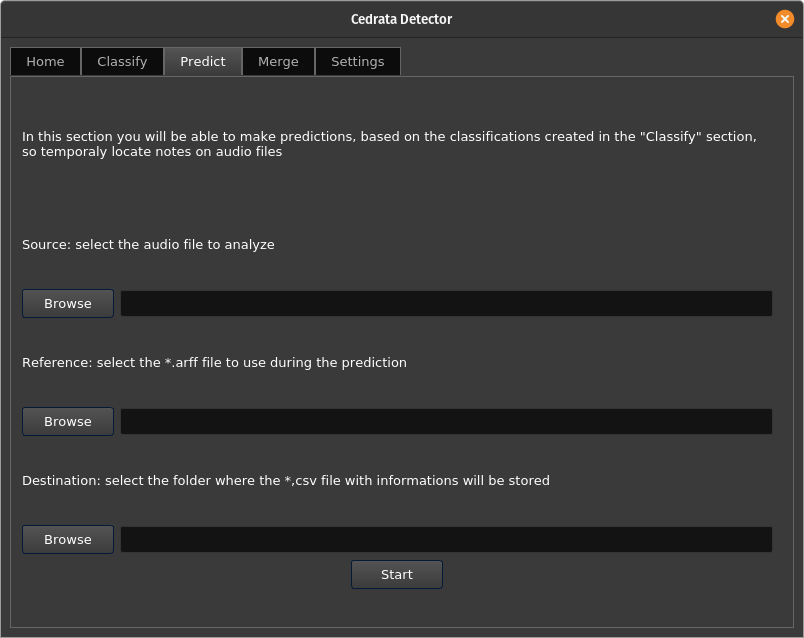
\includegraphics[scale=0.5]{./immagini/gui/predict.png}
	\end{center}
	\caption{Schermata di home}\label{fig:gui-predict}
\end{figure}

\section{Merge}
Questo progetto ha come obiettivo il fornire un modo per confrontare il tempismo tra i diversi strumenti e musicisti, ma i risultati ottenuti ora forniscono una visione per i singoli strumenti. Per avere una panoramica la soluzione adottata è stata quella di effettuare un merge di molteplici file, in un unico CSV. Questo è il compito di questa tab, è dunque , selezionare più risultati CSV di strumenti diversi appartenenti che suonano la stessa canzone, e specificare dove si vuole salvare il risultato. A questo punto si avrà un file contenente la colonna dei sample e per ogni strumento a ogni sample viene associato il valore da 1 a 5.
\begin{figure}[h!]
	\begin{center}
		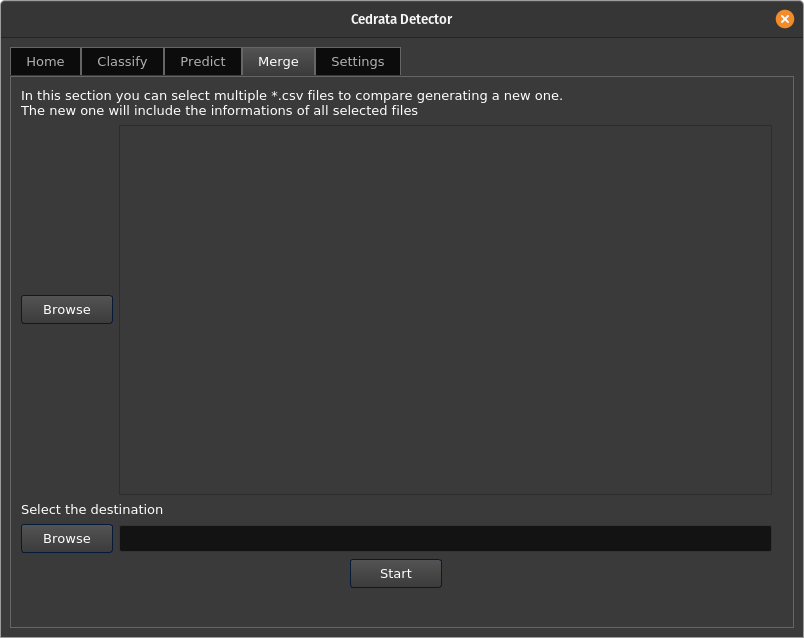
\includegraphics[scale=0.5]{./immagini/gui/merge.png}
	\end{center}
	\caption{Schermata di home}\label{fig:gui-merge}
\end{figure}


\section{Settings}
A differenza degli esperimenti, nei quali sono stati utilizzati dei parametri di riferimento descritti nel terzo capitolo, è fondamentale che un utente possa provare differenti configurazioni e impostazioni per portare a termine la configurazione e predizione. Per le due sezioni appena citate sono presenti due gruppi di impostazioni separati con gli stessi elementi: la selezione, tramite checkbox, delle features da utilizzare (media, varianza, media della derivata prima e seconda) la selezione della lunghezza di ogni sub-sample e il tempo di overlap che si vuole tra un sub-sample e l'altro. Sono stati inseriti poi i bottoni per applicare le impostazioni e ripristinare a default.
\begin{figure}[h!]
	\begin{center}
		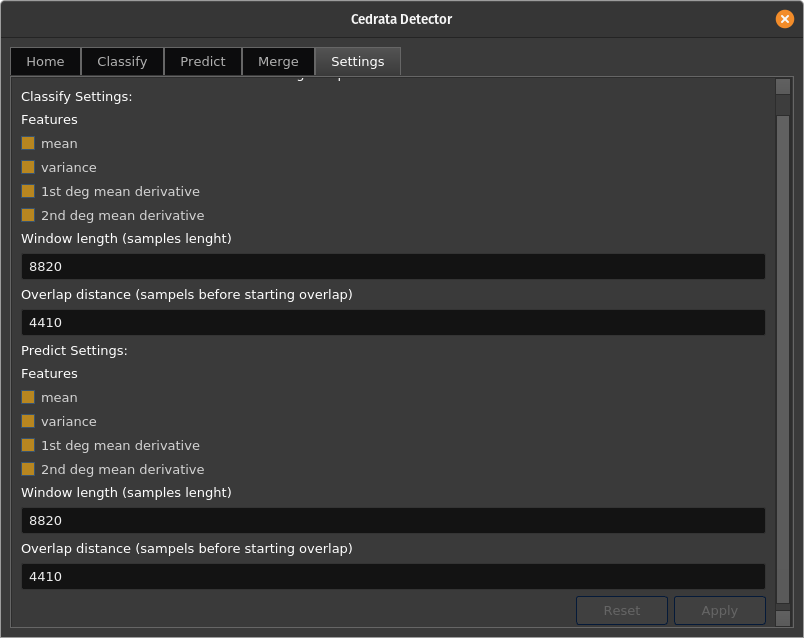
\includegraphics[scale=0.5]{./immagini/gui/settings.png}
	\end{center}
	\caption{Schermata di home}\label{fig:gui-settings}
\end{figure}